\documentclass{article}
\usepackage{float}
\usepackage[utf8]{vietnam}
\usepackage[english]{babel}
\usepackage[usenames,svgnames,dvipsnames]{xcolor}
\usepackage{tocloft}
\usepackage{booktabs}
\usepackage{siunitx}



\usepackage{tocloft}

% Change the title of the table of contents
\renewcommand{\contentsname}{Table of Contents}

% Change the font of the section titles
\renewcommand{\cftsecfont}{\bfseries}

% Change the font of the page numbers
\renewcommand{\cftsecpagefont}{\bfseries}

% Add a dot after the section numbers
\renewcommand{\cftsecaftersnum}{.}

% Change the indentation of the subsections
\setlength{\cftsubsecindent}{1cm}

%Fill with dots
\renewcommand{\cftsecleader}{\cftdotfill{\cftdotsep}}





\usepackage{amsmath}
\usepackage{listings}
\usepackage{xcoffins,calc}
\usepackage{amsthm}
\usepackage{amsfonts}
\usepackage{amssymb}
\usepackage{graphicx}
\usepackage{yhmath}
\usepackage{hyperref}
\usepackage[left=3.00cm, right=2.00cm, top=2.00cm, bottom=2.00cm]{geometry}
%\usepackage[amsthm]{ntheorem}
%\renewcommand\thechapter{\Roman{chapter}}
\renewcommand\thesection{\arabic{section}}
\theoremstyle{definition}
\newtheorem{bt}{Bài}

%\theoremstyle{nonumberplain}
%\theoremstyle{break}
%\numberwithin{equation}{chapter}
\usepackage{ esint }
\usepackage{array}
\usepackage{enumerate} 
%\usepackage{enumitem}
\usepackage{array}
\usepackage{longtable}
\usepackage{tikz}
\usetikzlibrary{graphs,graphs.standard}
\usepackage{tkz-euclide,amsmath}
\usepackage{ifthen}
\usepackage{mathrsfs}
\usetikzlibrary{arrows}
\pagestyle{empty}
\pagestyle{plain}
\usepackage{ mathrsfs } %chữ in hoa
%  \usepackage{pageborder} %khung bìa
\usepackage[utf8]{inputenc} 


\usetikzlibrary{arrows,%
                shapes,positioning}
                

\usetikzlibrary{calc}
\usepackage{longfbox}
\usepackage{indentfirst}
\usepackage{pgfplots}
\pgfplotsset{compat=1.15}
\usepackage{mathrsfs}
\usepackage{tikz}
\usepackage[most]{tcolorbox}
\usepackage{sectsty}


\usepackage[Glenn]{fncychap}
\let\svlim\lim\def\lim{\svlim\limits}
\newcommand\N{\ensuremath{\mathbb{N}}}
\newcommand\R{\ensuremath{\mathbb{R}}}
\newcommand\Z{\ensuremath{\mathbb{Z}}}
\renewcommand\O{\ensuremath{\emptyset}}
\newcommand\Q{\ensuremath{\mathbb{Q}}}
\newcommand\C{\ensuremath{\mathbb{C}}}
\renewcommand\P{\ensuremath{\mathcal{P}}}
\newcommand\V{\ensuremath{\nu}}

\let\implies\Rightarrow
\let\impliedby\Leftarrow
\let\iff\Leftrightarrow
\let\epsilon\varepsilon


% Setup for some boxes used in courses

\definecolor{gree}{RGB}{7, 135, 44}
%%%%%%%%%%%%%%%%%%%%%%%%%%%%%%%%%%%%%%%%%%%%%%%%%%%%

\newtcolorbox{claim}{
    enhanced,
    boxrule=0pt,frame hidden,
    borderline west={2pt}{0pt}{green!50!black},
    colback=green!10!white,
    sharp corners
}

\newtcolorbox{remark}{
    enhanced,
    boxrule=0pt,frame hidden,
    borderline west={4pt}{0pt}{black},
    colback=black!10!white,
    sharp corners
}

\newcommand{\Claim}{\textbf{\textcolor{green!50!black}{Claim -- }}}

\newcommand{\Remark}{\textbf{Why? -- }}

\usepackage{thmtools}
\usepackage[framemethod=TikZ]{mdframed}

\theoremstyle{definition}
\mdfdefinestyle{mdbluebox}{%
    roundcorner = 10pt,
    linewidth=1pt,
    skipabove=12pt,
    innerbottommargin=9pt,
    skipbelow=2pt,
    nobreak=true,
    linecolor=blue,
    backgroundcolor=TealBlue!5,
}
\declaretheoremstyle[
headfont=\sffamily\bfseries\color{MidnightBlue},
mdframed={style=mdbluebox},
headpunct={\\[3pt]},
postheadspace={0pt}
]{thmbluebox}

\declaretheorem[%
style=thmbluebox,name=Theorem,numberwithin=section]{theorem}
\declaretheorem[style=thmbluebox,name=Bổ đề,sibling=theorem]{lemma}
\declaretheorem[style=thmbluebox,name=Proposition,sibling=theorem]{proposition}
\declaretheorem[style=thmbluebox,name=Corollary,sibling=theorem]{corollary}

%%%%%%%%%%%%%%%%%%%%%%%%%%%%%%%%%%%%%%%%%%%%%%%%%%%%%

\usepackage{import}
\usepackage{xifthen}
\usepackage{pdfpages}
\usepackage{transparent}

\newcommand{\incfig}[1]{%
    \def\svgwidth{\columnwidth}
    \import{./figures/}{#1.pdf}
}
\newcommand{\kt}{\hfill{$\square$}}

\definecolor{atomkeywords}{rgb}{0.55, 0.47, 0.68}
\definecolor{atomstrings}{rgb}{0.78, 0.63, 0.45}
\definecolor{atomnumbers}{rgb}{0.5,0.5,0.5}
\definecolor{atomcomments}{rgb}{0.5, 0.5, 0.5}
\definecolor{atomoperators}{rgb}{0.4, 0.4, 0.4}
\definecolor{atombackground}{rgb}{0.95, 0.95, 0.95}
\definecolor{atomfunctions}{rgb}{0.4, 0.6, 0.8}

\lstdefinestyle{atomOneLight}{
    language=python,
    backgroundcolor=\color{atombackground},   
    commentstyle=\color{atomcomments},
    keywordstyle=\color{atomkeywords},
    numberstyle=\tiny\color{atomnumbers},
    stringstyle=\color{atomstrings},
    basicstyle=\ttfamily\footnotesize,
    breakatwhitespace=false,         
    breaklines=true,                 
    captionpos=b,                    
    keepspaces=true,                 
    numbers=left,                    
    numbersep=5pt,                  
    showspaces=false,                
    showstringspaces=false,
    showtabs=false,                  
    tabsize=2,
    classoffset=1,
    %%The below keywords will be highlighted in the code snippet.
    morekeywords={factorial, is_even, is_odd, tail_factorial, knapSack, fibonacci, tree, max, visit},
    keywordstyle=\color{atomfunctions},
    classoffset=0
}

\lstset{style=atomOneLight}


\begin{document}
\begin{titlepage}

\newcommand{\HRule}{\rule{\linewidth}{0.5mm}} % Defines a new command for the horizontal lines, change thickness here

\center % Center everything on the page
 
%----------------------------------------------------------------------------------------
%   HEADING SECTIONS
%----------------------------------------------------------------------------------------

\textsc{\LARGE VNU-HCM University of Science}\\[1.5cm] % Name of your university/college

\includegraphics[scale=.1]{logo.png}\\[1cm] % Include a department/university logo - this will require the graphicx package
\textsc{\Large Data Structure}\\[0.5cm] % Major heading such as course name
\textsc{\large CS163}\\[0.5cm] % Minor heading such as course title

%----------------------------------------------------------------------------------------
%   TITLE SECTION
%----------------------------------------------------------------------------------------

\HRule \\[0.4cm]
{ \huge \bfseries \uppercase{Articulation Points and Bridges}}\\[0.4cm] % Title of your document
\HRule \\[1.5cm]
 
%----------------------------------------------------------------------------------------
%   AUTHOR SECTION
%----------------------------------------------------------------------------------------

\begin{minipage}{0.4\textwidth}
\begin{center} \large

\emph{23APCS02}\\

Pham Gia Hung Khoa\\
Pham Nguyen Anh Tai\\

\end{center}

\end{minipage}\\[2cm]

% If you don't want a supervisor, uncomment the two lines below and remove the section above
%\Large \emph{Author:}\\
%John \textsc{Smith}\\[3cm] % Your name

%----------------------------------------------------------------------------------------
%   DATE SECTION
%----------------------------------------------------------------------------------------
\vfill % Fill the rest of the page with whitespace

{\large \begin{otherlanguage}{english}\today\end{otherlanguage}}\\[2cm] % Date, change the \today to a set date if you want to be precise




\end{titlepage}

\begin{otherlanguage}{english}\tableofcontents\end{otherlanguage}

\newpage

\section{Introduction}

In graph theory, understanding the structural integrity of networks is crucial. Bridges are edges whose removal increases the number of disconnected components in a graph, acting as critical links. Articulation points are vertices that, if removed, also increase the number of disconnected components, serving as essential hubs. Identifying these elements helps improve network design and resilience, whether in communication networks, transportation systems, social networks, or biological systems. By pinpointing these vulnerabilities, we can create more robust and efficient networks across various domains.\\
\section{Identifying Bridges and Articulation Points}

\subsection{Naive algorithm $O(NM)$}

For each edge $e \in E$, remove it from the graph and count the number of connected components $C'$, if $C' > C$ (the initial number of connected components), then we can claim that $e$ is a bridge, otherwise it is not a bridge.\\

The similar algorithm for finding the articulation points, which tests each removal of the vertex $v$, whether it increases the number of connected components of the graph. Which results in a $O(N^2)$ time complexity.\\

\textbf{\emph{Can we do better?}}
\subsection{DFS Tree}

To understand how we can effectively find the bridges and articulation points in terms of time complexity, we need to dive into the concept of DFS Tree.\\

Without loss of generality, let's assume that the graph $G$ is connected. In general, DFS Tree is a spanning tree of the graph when we do the DFS traversal of the graph.\\

Consider an undirected connected graph $G$. Let's run a depth-first traversal of the graph. It can be implemented by a recursive function like this:

\begin{lstlisting}
    function visit(u)
        mark u as visited
        for each vertex v among the neighbours of u:
            if v is not visited:
                mark the edge u-v
                invoke visit(v)
\end{lstlisting}

[animation and demonstration]\\

\newpage

This is the DFS tree of our graph:

\begin{figure}[H]

\centering
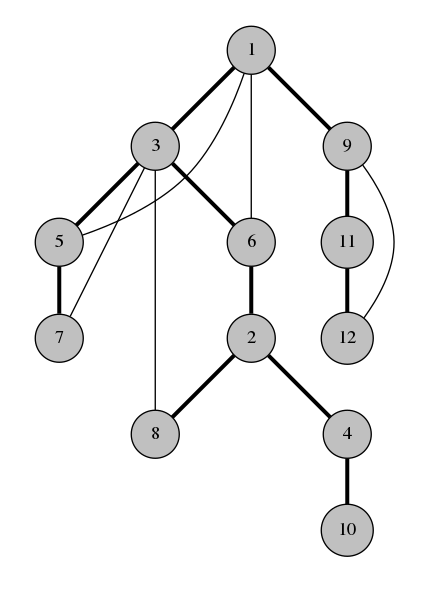
\includegraphics[scale=.5]{dfstreeDemo.png}\\[0.2cm] % 
\caption{DFS Tree Illustration.}

\end{figure}

Let's look at all edges that were marked in line 5. They form a spanning tree of $G$, rooted at the vertex 1. We will call these edges \emph{span-edges}, all other edges are \emph{back-edges}.\\

Then we have the following observation:\\

\textbf{Observation:} The back-edges of the graph all connect a vertex with its descendant in the spanning tree. \textbf{This is why DFS tree is so useful.}

\begin{remark}
    \Remark Suppose that there is an edge $uv$, and without loss of generality the depth-first traversal reaches $u$ while $v$ is still unexplored. Then:
    \begin{enumerate}[$\bullet$]
        \item If the depth-first traversal goes to $v$ from $u$ using $uv$, then $uv$ is a span-edge.

        \item If the depth-first traversal doesn't go to $v$ from $u$ using $uv$, then $v$ was already visited when the traversal looked at it at step 4. Thus it was explored while exploring one of the other neighbours of $u$, which means that $v$ is a descendent of $u$ in the DFS tree.
    \end{enumerate}
 \end{remark}

For example in the graph above, vertices 4 and 8 couldn't possibly have a back-edge connecting them because neither of them is an ancestor of the other. If there was an edge between 4 and 8, the traversal would have gone to 8 from 4 instead of going back to 2.

This is the most important observation about the DFS tree. The DFS tree is so useful because it simplifies the structure of a graph. Instead of having to worry about all kinds of edges, we only need to care about a tree and some additional ancestor-descendant edges. This structure is so much easier to think and write algorithms about.

\subsection{How to find Bridges and Articulation Points}

From this observation, we can come up with the following intuitive dynamic programming algorithm:

Let $dp[u] = \# \textit{of back-edges that connects $u$ or its descendants to its ancestors}$, then $dp[u]$ can be calculated using this formula:

\begin{align*}
    dp[u] &= \textit{\# of back-edges going from u to its ancestors }\\
            &- \textit{\# of back-edges going from u to its descendants } + \sum_{v \in child(u)} dp[v] 
\end{align*}

Using this definition of dynamic programming approach, we can check if an edge u->v in DFS tree is a bridge or not by checking whether $dp[v] = 0$. If it is true, then u->v is a bridge, otherwise it is not.\\

The same techniques can be used to check whether a vertex $v$  is an articulation point or not by checking the condition $dp[v] = 0$. But there is a special case that $v$ is the root of the DFS Tree, in which $dp[root]$ is always equal to 0, then we must check whether the root contains at least two children.

\subsection{Tarjan's Algorithm}

\subsubsection{Robert Tarjan}
Robert Endre Tarjan is an American computer scientist renowned for his contributions to the field of algorithms and data structures. He has made significant advances in graph theory, network analysis, and optimization, many of which are foundational in both theoretical and applied computer science. Tarjan is particularly famous for his development of efficient graph algorithms, some of which are used to solve problems like finding strongly connected components, shortest paths, and minimum spanning trees.

\subsubsection{The algorithm}
Tarjan suggested a more formal algorithm to find the articulation points and bridges. The algorithm based firmly on the previous observation:

\begin{enumerate}[$\bullet$]
    \item $num[u] =$ The first time it is visited by the DFS.
    \item $low[u] =$ The mininum of $num[u]$ that can be reached by going from u to any node in its sub-trees and using \textbf{at most one} back-edge.
\end{enumerate}

To calculate these two 2 arrays, we will use Depth-first Search technique to calculate it as follows:

\begin{enumerate}[$\bullet$]
    \item $num[u]$ will be calculated using a timer, or a variable called $cnt$. This timer will increase by one whenever we invoke a step of $dfs()$. We set $num[u] = ++cnt$
    \item Initially: $low[u] = num[u]$. For each edge $(u, v)$ (v is not parent of u):
    \begin{enumerate}
        \item If $(u, v)$ is a span-edge: $low[u] = min(low[u], low[v])$
        \item If $(u, v)$ is a back-edge: $low[u] = min(low[u], num[v])$
    \end{enumerate}
\end{enumerate}

After computing the $num$ and $low$ arrays, we could identify the bridges and articulation points in our graph:

\begin{claim}
    \begin{enumerate}[$\bullet$]
        \item A span-edge $(u, v)$ ($u$ is parent of $v$ in DFS Tree) is a bridge if $low[v] > num[u]$ (or $low[v] = num[v]$ or $low[v] >= num[v]$).
        \item A vertex $u$ is a cut if $low[v] \geq num[u]$ for any span-edge $(u, v)$.
    \end{enumerate}
\end{claim}


\section{Applications}
\subsection{Network Reliability and Vulnerability Analysis}

\textbf{Bridges:} Identifying bridges helps in understanding critical connections whose failure would disrupt network connectivity.\\

\textbf{Articulation Points:} Identifying these points helps in determining critical nodes whose failure would fragment the network.\\

Therefore, by understanding how weak or strong one network is, we could reinforce it via redundant paths or nodes to improve its fault tolerance, thus ensuring connectivity within the network itself.

\subsection{Transportation Networks}
\textbf{Infrastructure Planning:} Identifying bridges and articulation points in transportation networks (e.g., roads, railways) helps in planning for alternative routes and ensuring smooth transportation even if some parts of the network fail.\\

\textbf{Emergency Response:} Critical nodes and edges can be prioritized for maintenance and quick repairs to minimize disruption during emergencies.\\

\section{Additional Insights}

\subsection{Biconnected Components}
A Biconnected Component (BCC) in a graph is a maximal subgraph in which any two vertices are connected by at least two disjoint paths. This means that there are no single vertices whose removal would disconnect the subgraph. In other words, a BCC is a portion of the graph where connectivity is maintained even if any one vertex is removed.

\subsection{Block-cut Tree}
 Block-Cut Tree (BCT) is a tree structure that represents the decomposition of a graph into its biconnected components (blocks) and articulation points (cut vertices). In this tree, each block and each cut vertex is a node. Edges in the Block-Cut Tree connect cut vertices to the blocks they belong to, providing a clear hierarchical view of the graph's connectivity

\subsection{Two-edge Connected Component}
A two-edge connected component (also known as a 2-edge-connected component) in a graph is a maximal subgraph in which any two vertices are connected by at least two edge-disjoint paths. This means that there is no single edge whose removal would disconnect the subgraph.

\textbf{A Bridge Tree} is a tree structure derived from a graph, \textbf{where each node represents a two-edge connected component (2ECC)} of the original graph, and edges between nodes in the tree correspond to bridges (cut-edges) in the original graph that connects these components.

\subsection{Online Bridges}
Bridges can be found at the time of building the graph by the following idea:

\begin{enumerate}[$\bullet$]
    \item Initially we have the graph of n vertices and no edges.
    \item For each edge (u, v) to be added there can be 3 cases:
    \begin{enumerate}
        \item u and v are in the same 2-edges-connected component: The number of bridges does not change.
        \item u and v are in completely different components: The number of bridges increases by one.
        \item u and v are in the same connected component but different 2-edge-connected component: Creates cycle with one or more previous bridges. The number of bridges decreases by one or more
    \end{enumerate}
\end{enumerate}

\section{Reference}



\end{document}

